\documentclass{standalone}
\usepackage{tikz}
\usetikzlibrary{patterns, positioning}
\usepackage[sfdefault]{ClearSans} %% option 'sfdefault' activates Clear Sans as the default text font
\usepackage[T1]{fontenc}

\begin{document}
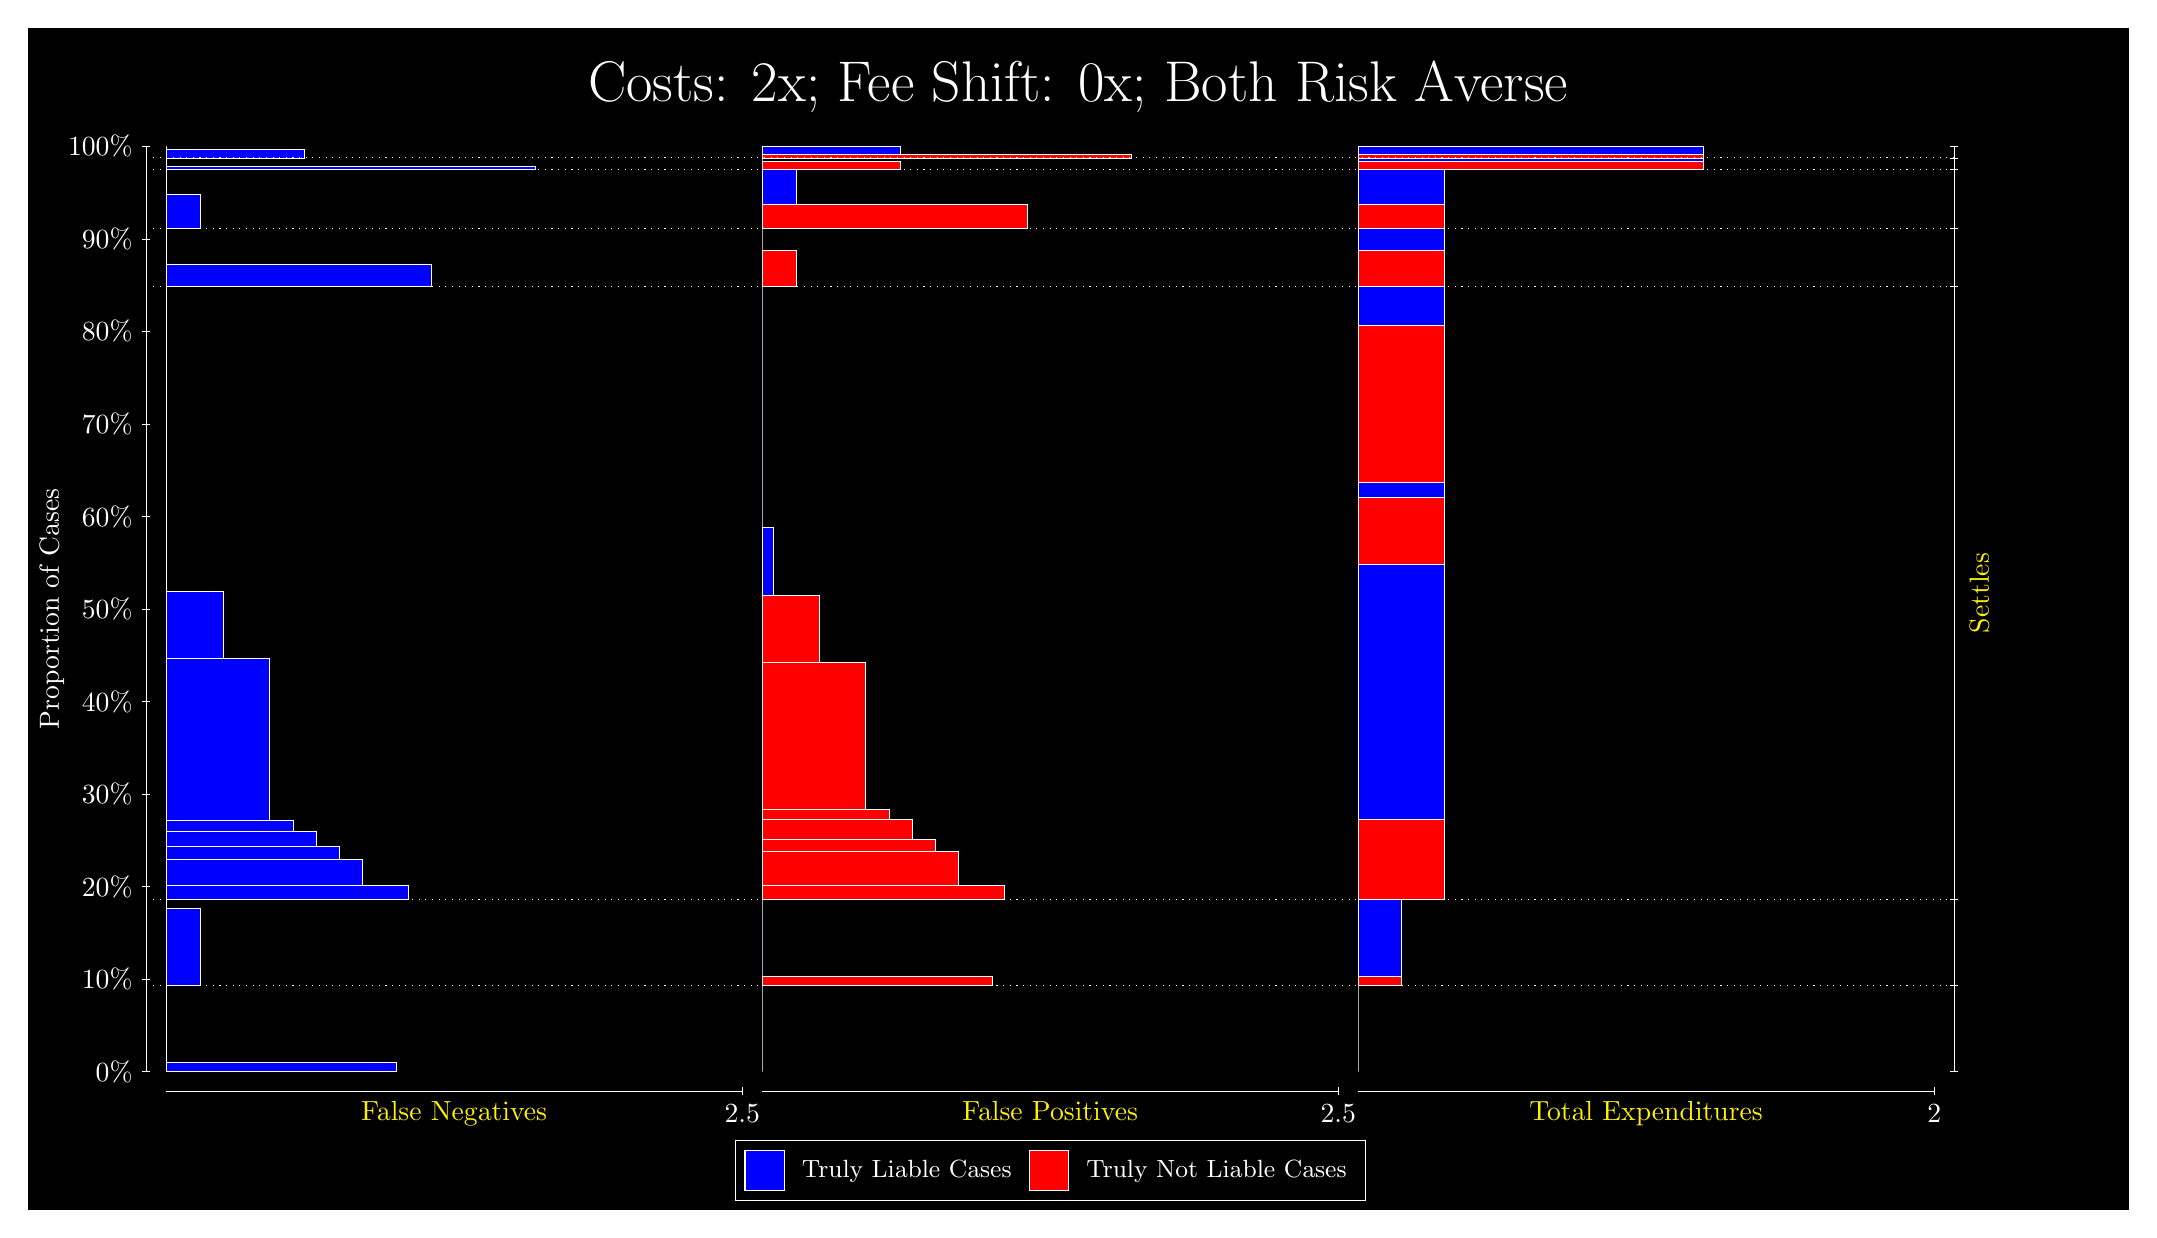
\begin{tikzpicture}
\draw[fill=black] (0,0) rectangle (26.667,15);
\draw[text=white] (0,13.5) rectangle (26.667,15) node[midway] {\huge Costs: 2x; Fee Shift: 0x; Both Risk Averse};
\draw[white, very thin] (1.5,1.75) -- (1.5,13.5);
\node[rotate=90, text=white, anchor=center] at (0.3, 7.625) {Proportion of Cases};
\draw[white, very thin] (1.45,1.75) -- (1.55,1.75);
\node[text=white, anchor=east] at (1.45, 1.75) {0\%};
\draw[white, very thin] (1.45,2.925) -- (1.55,2.925);
\node[text=white, anchor=east] at (1.45, 2.925) {10\%};
\draw[white, very thin] (1.45,4.1) -- (1.55,4.1);
\node[text=white, anchor=east] at (1.45, 4.1) {20\%};
\draw[white, very thin] (1.45,5.275) -- (1.55,5.275);
\node[text=white, anchor=east] at (1.45, 5.275) {30\%};
\draw[white, very thin] (1.45,6.45) -- (1.55,6.45);
\node[text=white, anchor=east] at (1.45, 6.45) {40\%};
\draw[white, very thin] (1.45,7.625) -- (1.55,7.625);
\node[text=white, anchor=east] at (1.45, 7.625) {50\%};
\draw[white, very thin] (1.45,8.8) -- (1.55,8.8);
\node[text=white, anchor=east] at (1.45, 8.8) {60\%};
\draw[white, very thin] (1.45,9.975) -- (1.55,9.975);
\node[text=white, anchor=east] at (1.45, 9.975) {70\%};
\draw[white, very thin] (1.45,11.15) -- (1.55,11.15);
\node[text=white, anchor=east] at (1.45, 11.15) {80\%};
\draw[white, very thin] (1.45,12.325) -- (1.55,12.325);
\node[text=white, anchor=east] at (1.45, 12.325) {90\%};
\draw[white, very thin] (1.45,13.5) -- (1.55,13.5);
\node[text=white, anchor=east] at (1.45, 13.5) {100\%};

\draw[white, very thin] (24.457,1.75) -- (24.457,13.5);
\draw[white, very thin] (24.407,1.75) -- (24.507,1.75);
\node[anchor=west] at (24.407, 1.75) {};
\draw[white, very thin] (24.407,2.8432) -- (24.507,2.8432);
\node[anchor=west] at (24.407, 2.8432) {};
\draw[white, very thin] (24.407,3.9336) -- (24.507,3.9336);
\node[anchor=west] at (24.407, 3.9336) {};
\draw[white, very thin] (24.407,11.721) -- (24.507,11.721);
\node[anchor=west] at (24.407, 11.721) {};
\draw[white, very thin] (24.407,12.46) -- (24.507,12.46);
\node[anchor=west] at (24.407, 12.46) {};
\draw[white, very thin] (24.407,13.203) -- (24.507,13.203);
\node[anchor=west] at (24.407, 13.203) {};
\draw[white, very thin] (24.407,13.354) -- (24.507,13.354);
\node[anchor=west] at (24.407, 13.354) {};
\draw[white, very thin] (24.407,13.5) -- (24.507,13.5);
\node[anchor=west] at (24.407, 13.5) {};

\draw[white, very thin, fill=blue] (1.75,1.75) rectangle (4.6775,1.865);
\draw[white, very thin, fill=red] (1.75,1.865) rectangle (1.75,2.8432);
\draw[white, very thin, fill=blue] (1.75,2.8432) rectangle (2.1891,3.8199);
\draw[white, very thin, fill=red] (1.75,3.8199) rectangle (1.75,3.9336);
\draw[white, very thin, fill=blue] (1.75,3.9336) rectangle (4.8239,4.1197);
\draw[white, very thin, fill=blue] (1.75,4.1197) rectangle (4.2384,4.4504);
\draw[white, very thin, fill=blue] (1.75,4.4504) rectangle (3.9457,4.6116);
\draw[white, very thin, fill=blue] (1.75,4.6116) rectangle (3.6529,4.806);
\draw[white, very thin, fill=blue] (1.75,4.806) rectangle (3.3602,4.9416);
\draw[white, very thin, fill=blue] (1.75,4.9416) rectangle (3.0674,6.9976);
\draw[white, very thin, fill=blue] (1.75,6.9976) rectangle (2.4819,7.8523);
\draw[white, very thin, fill=red] (1.75,7.8523) rectangle (1.75,11.721);
\draw[white, very thin, fill=blue] (1.75,11.721) rectangle (5.1167,12.002);
\draw[white, very thin, fill=red] (1.75,12.002) rectangle (1.75,12.46);
\draw[white, very thin, fill=blue] (1.75,12.46) rectangle (2.1891,12.897);
\draw[white, very thin, fill=red] (1.75,12.897) rectangle (1.75,13.203);
\draw[white, very thin, fill=blue] (1.75,13.203) rectangle (6.4341,13.246);
\draw[white, very thin, fill=red] (1.75,13.246) rectangle (1.75,13.354);
\draw[white, very thin, fill=blue] (1.75,13.354) rectangle (3.5065,13.457);
\draw[white, very thin, fill=red] (1.75,13.457) rectangle (1.75,13.5);
\draw[white, very thin, fill=red] (9.3189,1.75) rectangle (9.3189,2.7282);
\draw[white, very thin, fill=blue] (9.3189,2.7282) rectangle (9.3189,2.8432);
\draw[white, very thin, fill=red] (9.3189,2.8432) rectangle (12.246,2.9568);
\draw[white, very thin, fill=blue] (9.3189,2.9568) rectangle (9.3189,3.9336);
\draw[white, very thin, fill=red] (9.3189,3.9336) rectangle (12.393,4.1196);
\draw[white, very thin, fill=red] (9.3189,4.1196) rectangle (11.807,4.5426);
\draw[white, very thin, fill=red] (9.3189,4.5426) rectangle (11.515,4.7038);
\draw[white, very thin, fill=red] (9.3189,4.7038) rectangle (11.222,4.9484);
\draw[white, very thin, fill=red] (9.3189,4.9484) rectangle (10.929,5.0841);
\draw[white, very thin, fill=red] (9.3189,5.0841) rectangle (10.636,6.9474);
\draw[white, very thin, fill=red] (9.3189,6.9474) rectangle (10.051,7.8022);
\draw[white, very thin, fill=blue] (9.3189,7.8022) rectangle (9.4652,8.6569);
\draw[white, very thin, fill=blue] (9.3189,8.6569) rectangle (9.3189,11.721);
\draw[white, very thin, fill=red] (9.3189,11.721) rectangle (9.758,12.179);
\draw[white, very thin, fill=blue] (9.3189,12.179) rectangle (9.3189,12.46);
\draw[white, very thin, fill=red] (9.3189,12.46) rectangle (12.686,12.765);
\draw[white, very thin, fill=blue] (9.3189,12.765) rectangle (9.758,13.203);
\draw[white, very thin, fill=red] (9.3189,13.203) rectangle (11.075,13.311);
\draw[white, very thin, fill=blue] (9.3189,13.311) rectangle (9.3189,13.354);
\draw[white, very thin, fill=red] (9.3189,13.354) rectangle (14.003,13.397);
\draw[white, very thin, fill=blue] (9.3189,13.397) rectangle (11.075,13.5);
\draw[white, very thin, fill=red] (16.888,1.75) rectangle (16.888,2.7282);
\draw[white, very thin, fill=blue] (16.888,2.7282) rectangle (16.888,2.8432);
\draw[white, very thin, fill=red] (16.888,2.8432) rectangle (17.437,2.9568);
\draw[white, very thin, fill=blue] (16.888,2.9568) rectangle (17.437,3.9336);
\draw[white, very thin, fill=red] (16.888,3.9336) rectangle (17.986,4.9484);
\draw[white, very thin, fill=blue] (16.888,4.9484) rectangle (17.986,8.1891);
\draw[white, very thin, fill=red] (16.888,8.1891) rectangle (17.986,9.0438);
\draw[white, very thin, fill=blue] (16.888,9.0438) rectangle (17.986,9.2299);
\draw[white, very thin, fill=red] (16.888,9.2299) rectangle (17.986,11.229);
\draw[white, very thin, fill=blue] (16.888,11.229) rectangle (17.986,11.721);
\draw[white, very thin, fill=red] (16.888,11.721) rectangle (17.986,12.179);
\draw[white, very thin, fill=blue] (16.888,12.179) rectangle (17.986,12.46);
\draw[white, very thin, fill=red] (16.888,12.46) rectangle (17.986,12.765);
\draw[white, very thin, fill=blue] (16.888,12.765) rectangle (17.986,13.203);
\draw[white, very thin, fill=red] (16.888,13.203) rectangle (21.279,13.311);
\draw[white, very thin, fill=blue] (16.888,13.311) rectangle (21.279,13.354);
\draw[white, very thin, fill=red] (16.888,13.354) rectangle (21.279,13.397);
\draw[white, very thin, fill=blue] (16.888,13.397) rectangle (21.279,13.5);
\draw[white, dotted] (1.5,2.8432) -- (24.457,2.8432);
\draw[white, dotted] (1.5,3.9336) -- (24.457,3.9336);
\draw[white, dotted] (1.5,11.721) -- (24.457,11.721);
\draw[white, dotted] (1.5,12.46) -- (24.457,12.46);
\draw[white, dotted] (1.5,13.203) -- (24.457,13.203);
\draw[white, dotted] (1.5,13.354) -- (24.457,13.354);
\draw[white, very thin] (1.75,1.5) -- (9.0689,1.5);
\node[text=yellow, anchor=north] at (5.4094, 1.5) {False Negatives};
\draw[white, very thin] (9.0689,1.45) -- (9.0689,1.55);
\node[text=white, anchor=north] at (9.0689, 1.45) {2.5};

\draw[white, very thin] (9.3189,1.5) -- (16.638,1.5);
\node[text=yellow, anchor=north] at (12.978, 1.5) {False Positives};
\draw[white, very thin] (16.638,1.45) -- (16.638,1.55);
\node[text=white, anchor=north] at (16.638, 1.45) {2.5};

\draw[white, very thin] (16.888,1.5) -- (24.207,1.5);
\node[text=yellow, anchor=north] at (20.547, 1.5) {Total Expenditures};
\draw[white, very thin] (24.207,1.45) -- (24.207,1.55);
\node[text=white, anchor=north] at (24.207, 1.45) {2};



\node[text=yellow, centered, rotate=90] at (24.777, 7.8272) {Settles};





\draw (12.978300999999998,1.5) node[draw=none] (baseCoordinate) {};
\begin{scope}[align=center]
        \matrix[scale=0.5, draw=white, below=0.5cm of baseCoordinate, nodes={draw}, column sep=0.1cm]{
            \node[rectangle, draw, minimum width=0.5cm, minimum height=0.5cm, fill=blue] {}; &
            \node[draw=none, font=\small, text=white] (B) {Truly Liable Cases}; &
            \node[rectangle, draw, minimum width=0.5cm, minimum height=0.5cm, fill=red] {}; &
            \node[draw=none, font=\small, text=white] (B) {Truly Not Liable Cases}; \\
            };
\end{scope}

\end{tikzpicture}
\end{document}